\section{Passivity-Based Control} \label{section:pssivity}
\subsection{Mathematical Preliminaries}
Initial presentation of passive-decomposition is found in D. Lee et. al 2004. \cite{passive-decomp-mechanical-coord-req}. It decomposes the overall dynamics into shape system addressing the coordination aspect, locked system representing internal dynamics wrt. the holonomic constraints and dynamic couplings between the locked and shape systems.The coupled dynamics can be canceled out without violating passivity. Thus, the coordination aspect (shape system) and the dynamics of the coordinated (locked) system can be decoupled from each other while enforcing passivity. By designing the locked and shape controls to enforce passivity  of their respective systems, the closed-loop system energetic passivity is guaranteed. A brief introduction towards passive-decomposition is given as follows. \\
Consider a group of $m$-mechanical systems such that the $i$-th agent's dynamics evolve on a configuration manifold $\Ma_i$:
	\begin{equation}
	M_i(\textbf{q}_i)\nabla^i_{\textbf{v}_i} \textbf{v}_i = \textbf{T}_i + \textbf{F}_i, \;\;\; i = 1,...,m,
\end{equation}
where the following terms are defined as follows:
\begin{itemize}
	\item $\textbf{T}_i, \textbf{F}_i\in\text{T}_{\textbf{q}_i}^*\Ma_i$ - control and environmental force covectors that exist in a cotangent manifold at point $\textbf{q}_i$
	
	\item $\textbf{v}_i \in \text{T}_i^{*}\Ma_i$ - system velocity at point $\textbf{q}_i$ in the tangent manifold
	
	\item $\nabla^i_{\textbf{v}_i}$ - this symbol represents a covariant derivative operator, the Levi-Civita connection. It provides a well defined method of differentiating vector fields along the ${\textbf{v}_i}$ direction on the tangent bundle $\text{T}\Ma_i$.
	
	\item $M_i(\textbf{q}_i)$ - inertia tensor which maps vectors from tangent space to cotangent space at point $\textbf{q}$, defined as $M:\text{T}_{\textbf{q}}\Ma \mapsto \text{T}_{\textbf{q}}^*\Ma$
\end{itemize}

Furthermore, the supply rate for the m-agent mechanical system is defined as follows.
\begin{equation}
	s_\rho(\textbf{v}_i, \textbf{T}_i) = \langle\textbf{F}_i, \dot{\textbf{q}}_i \rangle + ... + \langle\textbf{F}_m, \dot{\textbf{q}}_m \rangle \, ,
\end{equation}
where $\langle \cdot, \cdot \rangle: \text{T}_{\textbf{q}}^*\Ma \times \text{T}_{\textbf{q}}\Ma  \rightarrow \mathbb{R}$. \\
\noindent For safe and stable interaction an energetic passivity condition where $\exists d\in\mathbb{R}$ such that: 
\begin{equation}
	 \int_{0}^{t}	s_\rho(\textbf{v}_i(\tau), \textbf{T}_i(\tau))d\tau \geq -d^2, \;\forall t\geq 0
\end{equation}
Similar condition is employed to induce controller passivity. \\
Introducing the coordination map $h:\Ma^n \rightarrow \Na^m$ which holds the holonomic constraints, at each point of the configuration manifold $q\in\Ma$, the corresponding tangent space $\text{T}_q\Ma$
is split into two orthogonal vector spaces as follows:
\begin{equation}
	\text{T}_q\Ma = \text{T}_q^\top \Ma \oplus \text{T}_q^{\perp} \Ma
\end{equation}
The tangential and perpendicular spaces are defined respectively:
\begin{gather}
	\text{T}_q^\top\Ma := span \{v \in \text{T}_q\Ma \, \vert \, h_*(v) = 0\}  \\
	\text{T}_q^\perp\Ma := span \{w \in \text{T}_q\Ma \, \vert \, \langle \langle v, w \rangle \rangle, \, \forall v \in \text{T}_q^\top \Ma  \}, 
\end{gather}
where $h_*: \text{T}_q\Ma \rightarrow \text{T}_{h(q)}\Na$ is a push-forward of the coordination map. \\
By applying the orthogonal decomposition to the model dynamics we are able to decouple the shape and locked dynamics, while applying a control law cancel the coupling which essentially sums up the notion of passive-decomposition.

\subsection{Trajectory Tracking}
A concrete application of the passive-decomposition concepts on a UAV system can be found in \cite{passive-decomp-quadrotor-with-robotic-manip}. The authors show that the Lagrange dynamics of quadrotor-manipulator systems can be completely decoupled into: the center-of-mass dynamics in E(3), which, similar to the standard quadrotor dynamics, is point-mass dynamics with under-actuation  and  gravity  effect; the  “internal rotational” dynamics  of  the  quadrotor’s  rotation  and  manipulator configuration, which assumes the form of standard Lagrange dynamics  of  robotic manipulator with full-actuation and nogravity effect.  
\begin{figure}[H]
	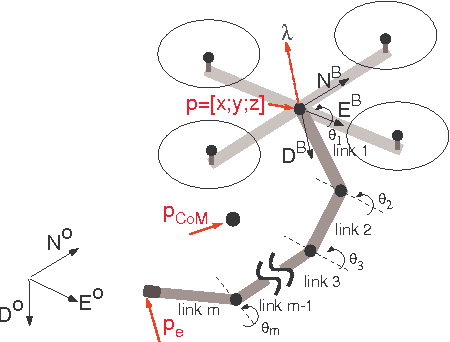
\includegraphics[width=0.95\columnwidth]{figure/aerial_manip.png}	
	\centering
	\caption{This $\text{figure}^{\cite{passive-decomp-quadrotor-with-robotic-manip}}$ represents a quadrotor UAV with a generalized m-DOF robot arm. The UAV platform's position is denoted with $\textbf{p}$, $\textbf{p}_e$ represents the end-effector position while $\textbf{p}_{CoM}$ is the center-of-mass vector of the entire quadrotor-manipulator system. It is worth nothing that a general case is considered where $\textbf{p}_{CoM} \neq\textbf{p}$.  }
	\label{fig:aerial_manip}
\end{figure}
\noindent A backstepping-like end-effector tracking control law is proposed, which allows  assignment of different roles for the center-of-mass control and internal rotational dynamics  control according to task objectives.

A similar passivity-based control design is presented in \cite{decoupled-aerial-manipulation} for quadrotor-manipulator UAV system utilizing a PID cascade  unlike the previously shown backstepping controller. Proposed control algorithms are implemented in the MATLAB/
Simulink environment and tested using the highly nonlinear system model in simulation. 
The controller robustness is checked by applying disturbance forces from different 
directions at the tip point of the 2-DOF robotic arm.

In \cite{passivity-backstepping}  a novel unified passivity-based adaptive backstepping control framework is proposed for ‘mixed’ quadrotor UAVs. It consists of the translation dynamics with thrust force input and the attitude kinematics with the angular velocity input evolving on SE(3). Its application to haptic teleoperation over the Internet is also presented with dynamic-extension like filter to address discontinuous communication and a complete stability/collision-avoidance analysis is provided.

\subsection{Payload Transportation}
As it was the case with geometric control methods, there are a multitude of applications of passivity-based control on payload carrying and transportation. In \cite{passivity-based-formation-load} the authors propose a strategy consisting of internal feedback control for each UAV and a general formation control law regulating relative positions between each UAV pair. It is proven that under such control strategy the system is stable for all equilibrium points where the cables supporting the suspended load are in tension. \\
\noindent Furthermore, the authors in \cite{passivity-based-payload-minimum-swing} present the Euler-Lagrange formulation quadrotor, cable and payload system. An Interconnection and Damping Assignment-Passivity Based Control (IDA-PBC) for a quadrotor UAV transporting a cable-suspended payload is developed. The designed method does not depend on the swing angle of the cable. Main control objective shown was to transport the payload from point to point, with swing suppression along the desired trajectory. \\ 
It is worth mentioning the research done in \cite{payload-and-human}. A novel concept of master-slave strategy is implemented where the  master  quadrotor  is  controlled  by a human  and  the slave quadrotor tries to stabilize the oscillations of the payload. Two  UAVs with a cable-suspended  payload  is an under-actuated system with coupled dynamics, therefore manual control is proven difficult. A Lyapunov based  controller is designed to  minimize  the  oscillations  of  the  payload while  transportation,  leading  to  an  easier  manual  control  of master quadcopter.

\subsection{Aerial Compliance}
As previously mentioned, one of the main motivations for implementing passive decomposition on UAV systems is to achieve compliant behavior. Research in \cite{passive-variable-impedance-compliant} concerns the notion of passivity-based compliant control methods. The authors introduce a novel scheme, termed Passivity-Preservation Control (PPC), which suppresses the energy injections that could be introduced into compliant robots, as a result of Variable Impedance Control (VIC). Although the presented controller is used with manipulators, this research is still worth mentioning as generally the notion of aerial compliance implies a manipulator endowed UAV. \\
Regarding quadrotors interacting with the environment, in \cite{quadrotor-itneraction-environment} a novel method for applying a wrench while flying is proposed. Inspired by the use of contacts in legged robots, the authors present an idea of exploiting physical contact with the environment, with the goal of going beyond the common thought that the surrounding environment is a constraint to avoid. \\
An energy conservative approach to maximum wrench generation by a fully actuated aerial robot is presented in \cite{max-wrench-min-energy}. Two different approaches for designing the rotor tilt angles of a fully actuated aerial robot are presented in this paper. A common approach is based on maximizing the forces and torques the robot can generate. To determine the tilt angles, simple knowledge of the maximum required wrench is necessary. Another approach focuses on following an a priori defined trajectory with minimum energy consumption, taking advantage of the nonlinear power-thrust characteristic of a real propeller. For this purpose, complex knowledge of the complete trajectory is necessary, especially for rotors with fixed orientation.   \\
A passivity-based control of a fully actuated UAV for aerial physical interaction near hovering is presented in \cite{passivity-based-physical-interaction}. A unified near-hovering motion and impedance controller is derived by the energy-balancing passivity-based control technique. A detailed analysis of the closed-loop system’s behavior  is presented for both the free-flight and contact stability of the UAV. Robustness of the control system to uncertainties is validated by several experiments, in which the UAV is controlled near its actuator limits.

\begin{figure}[H]
	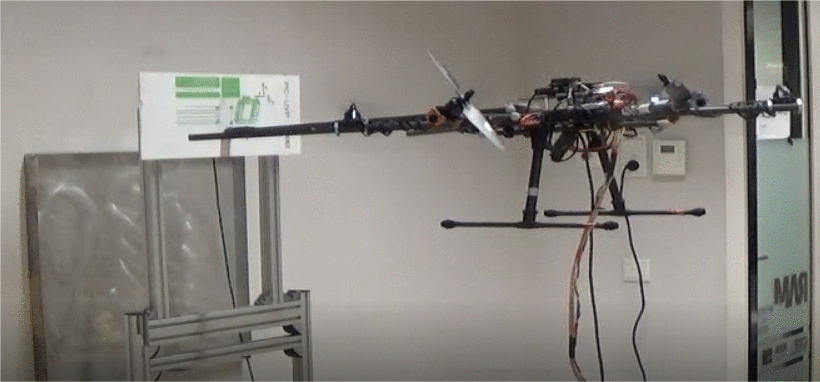
\includegraphics[width=0.95\columnwidth]{figure/passivity-based-interaction.png}	
	\centering
	\caption{This $\text{figure}^{\cite{passivity-based-physical-interaction}}$ represents a fully-actuated hexarotor UAV hovering with one rotor off and applying ~10N of force to a verticl surface rigidly connected to a force sensor.}
	\label{fig:aerial_compliance}
\end{figure}

Another example of aerial interaction is research presented in \cite{passivity-based-aerial-interaction}. The authors propose a novel control method based on interconnection and damping assignment passivity-based control (IDA-PBC) in order to address the aerial physical interaction (APhI) problem for a quadrotor unmanned aerial vehicle. The apparent physical properties of the UAV are reshaped in order to achieve better APhI performances, while ensuring the stability of the interaction through passivity preservation. The validity and practicability of the proposed APhI method is evaluated through experiments, where for the first time in the literature, a lightweight all-in-one low-cost force/torque (F/T) sensor is used onboard of a quadrotor. Two main scenarios are shown: a quadrotor responding to external disturbances while hovering (physical human–quadrotor interaction), and the same quadrotor sliding with a rigid tool along an uneven ceiling surface (inspection/painting-like task).

Lastly, it's worth mentioning an ongoing research project \cite{door-opening}. The authors set a goal of autonomous door opening with the Interacting-BoomCopter (I-BC) UAV. This paper presents the design of a light-weight, compliant end-effector and an image processing strategy that together enable the I-BC UAV to perform the task. 

\begin{figure}[H]
	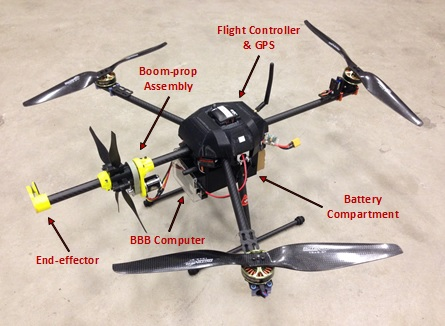
\includegraphics[width=0.95\columnwidth]{figure/BoomCopter.jpg}	
	\centering
	\caption{This $\text{figure}^{\cite{door-opening}}$ shows the \textit{BoomCopter} design by the RoSeHUB Research Laboratory at Purdue University. Equipped with boom-prop assembly it is able to perform various tasks physically interacting with environment, such as opening doors. }
	\label{fig:boom_copter}
\end{figure}

\subsection{Inspection Tasks}

Endowed with various sensor suites, tasks such as surveillance, inspection \cite{ref:corosion-inspection}\cite{ref:inspection-overview}\cite{Ollero2018}, search and rescue \cite{ref:sar}, 3D mapping \cite{ref:lidar-equipped-model-building}, etc. are well within  the operational reach.

In \cite{passivity-based-crop} the development of a passivity based visual servoing controller with dynamics compensation for the tracking of roads is presented. The proposed system allows the autonomous navigation of a UAV on straight lines such as those found in areas of structured crops. The stability of the controller is shown in the context of the input-output theory and based on the passivity properties of the system.

\begin{figure}[H]
	\centering
	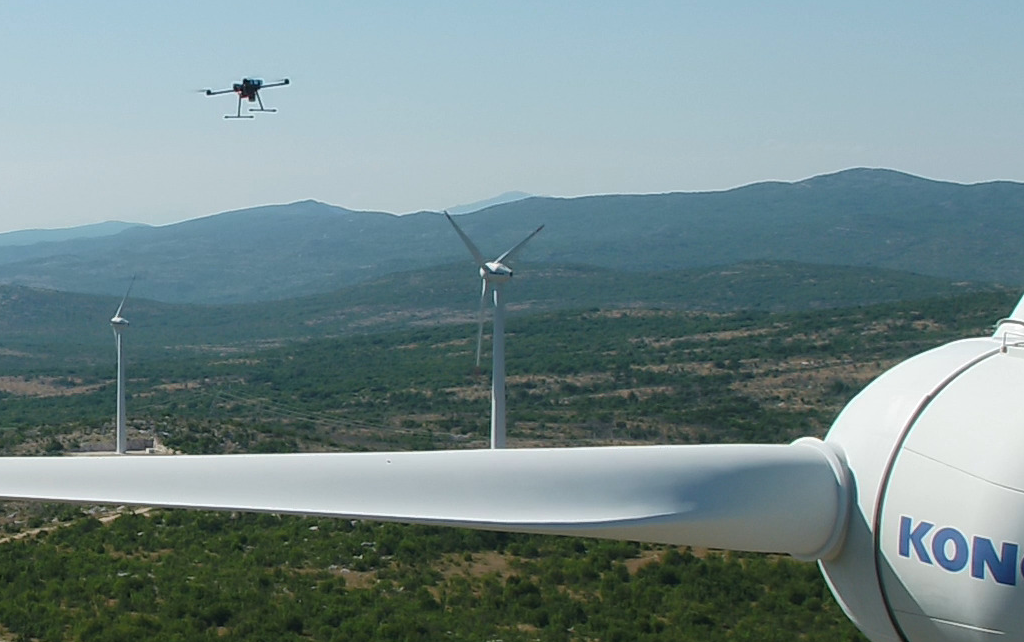
\includegraphics[width=\columnwidth]{./figure/drone_flight3_1.png}
	\caption{Custom built UAV equipped with a Velodyne VLP-16 LiDAR sensor filmed mid-flight  while performing a manually operated inspection procedure on a wind-turbine blade.}
	\label{fig:drone-flight}
\end{figure}


\subsection{Other Notable Contributions}
The paper \cite{passivity-attitude-sync} addresses passivity-based motion coordination of rigid bodies in the special Euclidean group SE(3) under the assumption that the agents exchange information over strongly connected graphs. A passivity-based distributed velocity input law to achieve attitude synchronization is developed. Using the notion of algebraic connectivity, a connection between the speed of convergence and the structure of the interconnection graph is established. Attitude synchronization in the leader-follower case and in the cases of communication delay and temporary communication failures is subsequently proven.

A hierarchical cooperative control framework for multiple quadrotor-manipulator systems is presented in \cite{cooperative-control-quadrotor}. It allows the endowment of a common grasped object with a user-specified desired behavior (e.g., trajectory tracking, compliant interaction, etc.). To achieve  this,  our  control  framework  con-sists  of  the  following  hierarchical  layers: 1) object desired behavior design; 2) optimal cooperative force distribution; 3)individual quadrotor-manipulator control based on object stiffness model, which can also take into account different dynamics characteristics of the (slower/coarser) quadrotor-platform and the (faster/finer) manipulator.

In \cite{group-teleoperation} an experimental validation of a novel decentralized passivity-based control strategy for teleoperating a group of Unmanned Aerial Vehicles (UAVs) is presented. The slave side, consisting of the UAVs, is endowed with large group autonomy by allowing time-varying topology and interrobot/obstacle collision avoidance. The master side, represented by a human operator, controls the group motion and receives suitable force feedback cues informing her/him about the remote slave motion status. Passivity theory is exploited for guaranteeing stability of the slave side and of the overall teleoperation channel.

A semi-autonomous haptic teleoperation control architecture for multiple UAVs is presented in \cite{haptic-teleoperation-uav}. It consist of three control layers: 1) UAV control layer where each UAV is abstracted and controlled to follow the trajectory of, its own kinematic Cartesian virtual point (VP); 2) VP control layer, which modulates each VP’s motion according to the teleoperation commands and local artificial potentials (for VP–VP/VP-obstacle collision avoidance and VP–VP connectivity preservation); and 3) teleoperation layer, through which a single remote human user can command all (or some) of the VPs’ velocity while haptically perceiving the state of all (or some) of the UAVs and obstacles. Master passivity/slave stability and some asymptotic performance measures are proven. 